\documentclass[10pt,notitlepage]{article}
\usepackage{graphicx} 
\usepackage{verbatim} 
\usepackage[portuguese]{babel} 
\usepackage[utf8]{inputenc}
\usepackage[hmargin=2cm,vmargin=3.5cm,bmargin=2cm]{geometry}


\begin{document}

%%%CAPA%%%
\begin{titlepage}
\begin{figure}
\centering

\includegraphics[scale=0.5]{logo.pdf}
\end{figure}



\begin{center}

Escola de Engenharia \\~  Departamento de Informática \\~ \\~ Licenciatura em Engenharia Informática \\~ \\~ \\~  \\~ \\~ \\~ \\~ \\~ \\~ \\~  


{\Huge Projecto Java - FitnessUM }
\\~ \\~ \\~ \\
Programação Orientada aos Objectos
  \vfill

\begin{figure}[h]
\centering

\end{figure}

\begin{figure}[h]
\centering
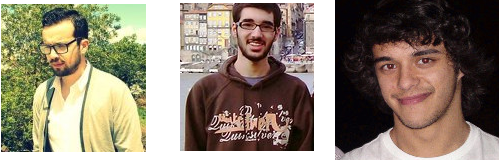
\includegraphics[scale=0.6]{autores.png}
\end{figure}

69854 ~~~~~~~~~~~~~~~~~~ 66822 ~~~~~~~~~~~~~~~~~~ 69303   \\~  João Mano ~~~~~~~~ Miguel Guimarães ~~~~~~~~ Bruno Torres  \\~ \\~ \\~ \\~ \\~ \\~ Braga, Junho de 2014
\end{center}
\end{titlepage}




\tableofcontents

\newpage


\section{Estrutura da aplicação}

\subsection{Actividades}
Foram definidas as seguindes actividades desportivas para a nossa aplicação:
\begin{itemize}
\item Yoga
\item Aerobics
\item Swimming
\item IndoorCycling
\item Handball
\item Basketball
\item TableTennis
\item Boxing
\item Badminton
\item VolleyBallIndoor
\item Football
\item VolleyBallBeach
\item Running
\item Skating
\item Saling
\item Walking
\item Tennis
\item Skiing
\item Cycling
\item MountainBiking
\item Orienteering
\item Snowboarding
\item Polo

\end{itemize}

\newpage
Para a implementação destas actividades foi usada a seguinte estrutura:

\begin{figure}[ht]
\centering
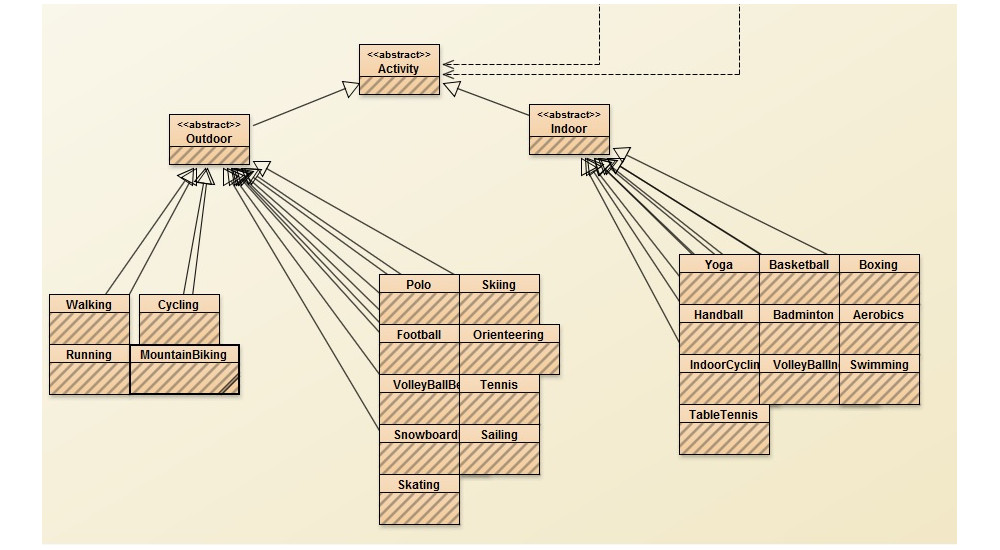
\includegraphics[scale=0.5]{Activity2.jpg}
\caption{Estrutura das actividades}
\label{fig:actividades}
\end{figure}


\subsubsection{Classe abstracta Activity}

Esta é a classe mais abstrata, que tem a fundação de todas as actividadades desta aplicação. Contém variáveis comuns a todas as actividades:

 \textit{name}, \textit{date}, \textit{timeSpent} e \textit{calories} tal como os construtores, \textit{getters} e  \textit{setters}.

\subsubsection{Indoor,Outdoor e actividades desportivas}
Todas as actividades desportivas tem um aspecto importante,o clima caso sejam praticadas ao ar livre.\\
Devido a este aspecto foram criadas duas classes abstractas,subclasses de \textit{Activity},para essa distinção.  
\begin{itemize}
\item Outdoor,contém a variável: \textit{String weather}  
\item Indoor
\end{itemize}

Todas as actividades desportivas são subclasses de \textit{Indoor} ou \textit{Outdoor} como exemplicado na figura ~\ref{fig:actividades}. 
\subsubsection{Comparadores}
Para organizar as actividades criaram-se dois tipo de comparadores:
\begin{itemize}
\item CompareActivity- Compara a actividade pela data da realização da mesma.
\item CompareActivityByTime- Compara a actividade pelo tempo gasto na realização desta.
\end{itemize}

\begin{figure}[ht]
\centering
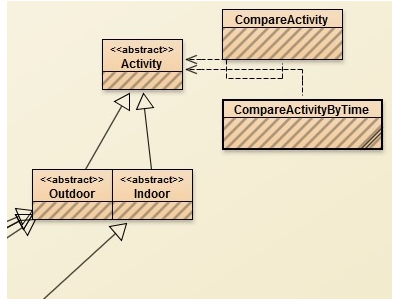
\includegraphics[scale=1]{ComparadorActivity.png}
\caption{Comparador Activity}
\end{figure}


\subsection{Utilizadores}

\begin{figure}[ht]
\centering
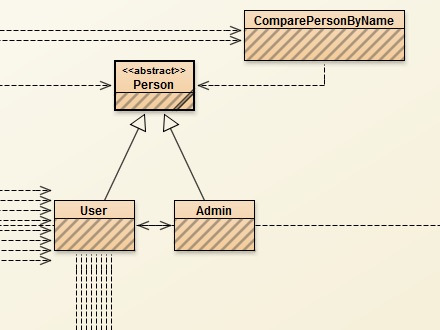
\includegraphics[scale=1]{Person.jpg}
\caption{Estrutura das classes User e Admin}
\end{figure}

\subsection{Classe Abstracta Person}

Aqui usámos mais uma classe abstracta para definir todas as pessoas que usam a aplicação (Administradores ou utilizadores normais). As variáveis comuns aos todos os tipos de pessoas são \textit{email}, \textit{password}, \textit{name}, \textit{gender}, e \textit{dateOfBirth}. Para além de 
construtores, \textit{getters} e \textit{setters} esta classe não tem métodos auxiliares.




\subsection{Eventos}

\subsection{Classe abstracta Event}

Classe com o conceito mais abstracto de Evento, contém as variáveis \textit{name}, \textit{tipoActivity}, \textit{location}, \textit{maxParticipants}, \textit{participants}, \textit{deadline}, \textit{date}, \textit{duration}, \textit{participantsList}, \textit{ranking}, \textit{desistentes} e \textit{simula}, respetivos \textit{getters} e \textit{setters} e os vários contrutores. Ainda tem métodos auxiliares para adicionar um \textit{User}, \textit{ranking}, 


\subsection{}


\end{document}

















